% =============================================================================
% RigorBench: Benchmarking Engineering Process Discipline
%             in Autonomous AI Coding Agents (Workshop Track)
% =============================================================================
\documentclass[letterpaper, 10 pt, conference]{ieeeconf} 
\IEEEoverridecommandlockouts  
\overrideIEEEmargins

\usepackage[utf8]{inputenc}
\usepackage[T1]{fontenc}
\usepackage{times}
\usepackage{pifont}
\usepackage{graphicx}
\usepackage{amsmath,amssymb}
\usepackage{booktabs}
\usepackage{multirow}
\usepackage{xcolor}
\usepackage{hyperref}
\usepackage{cleveref}
\let\labelindent\relax
\usepackage{enumitem}
\usepackage{tikz}
\usepackage{microtype}

\hypersetup{colorlinks=true, linkcolor={blue!70!black}, citecolor={green!50!black}, urlcolor={blue!60!black}}

\newcommand{\bench}{\textsc{RigorBench}}
\newcommand{\rigorscore}{\textsc{RigorScore}}
\newcommand{\pillar}[1]{\textsc{#1}}

\title{\LARGE \bf
  RigorBench: Probing the Over-Engineering Tax \\
  in Autonomous AI Coding Agents
}

\author{ \parbox{3 in}{ \centering Meher Bhaskar Madiraju
        {\tt\small meherbhaskar.madiraju@gatech.edu}}
        \hspace*{ 0.5 in}
        \parbox{3 in}{\centering Meher Sai Preetam Madiraju
        {\tt\small mehersaipreetam@gatech.edu}}
}

\begin{document}

\maketitle
\thispagestyle{empty}
\pagestyle{empty}

\begin{abstract}
Agentic coding harnesses are increasingly deployed for real-world software engineering tasks. Existing benchmarks evaluate these agents almost exclusively on outcome correctness: whether generated code passes tests or resolves issues. We argue this outcome-only lens is insufficient and hides a massive blindspot: an agent that arrives at a correct solution through reckless trial-and-error is fundamentally less reliable than one following sound engineering discipline. We introduce \bench{}, an exploratory benchmark measuring process discipline. To test whether process discipline can be measured and enforced, we developed Agent-Rigor not as a commercial competitor, but as an experimental probe hardcoded to enforce upfront planning and verification. Our goal is to observe how forcing process alters LLM execution trajectories. Our results reveal a paradoxical finding: enforcing macro-level discipline elevates a framework's overall capability ceiling (a 79\% improvement in process quality scores and 30\% increase in outcome correctness), yet fails to predict task-level success on individual runs ($r=0.12$). We invite the community to explore this "Over-Engineering Tax" where ReAct "cowboy coding" fails and structured planning becomes mathematically worth the overhead.
\end{abstract}

\section{Introduction \& Related Work}
The rapid maturation of large language models (LLMs) has given rise to the \emph{agentic coding harness}. Frameworks like Agent-Skills and Superpowers now operate with increasing autonomy. Their capabilities are evaluated by benchmarks like SWE-bench~\cite{jimenez2024swebench}, HumanEval~\cite{chen2021evaluating}, and BigCodeBench~\cite{zhuo2024bigcodebench}. 

These benchmarks share a common evaluation philosophy: they measure \emph{outcomes}. While outcome correctness is necessary, it is not sufficient for reliable deployment. Consider two agents: Agent A reads an error trace, formulates a hypothesis, writes a fix, and verifies it. Agent B tries five random patches in sequence until tests pass. Under existing benchmarks, both agents receive the same score. Yet their reliability profiles are radically different.

Decades of software engineering research---from Humphrey's Personal Software Process~\cite{humphrey1989managing} to the Capability Maturity Model Integration~\cite{cmmi2018}---have established that \emph{how} software is built predicts long-term quality. Emerging standards like the Linux Foundation AAIF AGENTS.md~\cite{linuxfoundation2024agentsmd} guide agent behavior through project-level hints, while Agent-Skills~\cite{osmani2024agentskills} and Superpowers~\cite{obra2024superpowers} natively augment the agent's action space. Despite this rich landscape, every benchmark evaluates \emph{what} the agent produces, not \emph{how} it produces it.

\section{The Process Discipline Gap}
We surveyed major AI coding benchmarks (HumanEval, SWE-bench, DevBench, AgentBench, etc.) and found that \emph{none} incorporate measurements of planning quality, verification behavior, recovery strategy, or codebase health maintenance. This gap has practical consequences: agents optimized purely for outcome metrics may develop strategies that are effective in the lab but hazardous in production. \bench{} is designed to detect and penalize exactly these anti-patterns, providing a complementary evaluation axis to existing benchmarks.

\section{RigorBench Design}
\bench{} is structured around three core decisions: (1) a seven-pillar scoring framework, (2) a curated 100-task suite, and (3) a trajectory-based evaluation methodology.

\subsection{The Seven Scoring Pillars}
Each pillar captures a distinct dimension of engineering discipline. A composite \rigorscore{} aggregates these dimensions into a single metric. (See Appendix A for formal mathematical scoring formulas and $\lambda$ decay parameters).
\begin{itemize}[leftmargin=*,itemsep=1pt]
  \item \pillar{Planning Fidelity (PF)}: Measures deliberate planning before code generation.
  \item \pillar{Verification Coverage (VC)}: Evaluates whether the agent verifies its own output through testing.
  \item \pillar{Recovery Efficiency (RE)}: Measures the agent's ability to recover from errors without entering doom loops.
  \item \pillar{Abstention Quality (AQ)}: Evaluates the agent's epistemic humility on impossible tasks.
  \item \pillar{Atomic Transition Integrity (ATI)}: Measures whether the codebase remains healthy between steps.
  \item \pillar{Test Assertion Density (TAD)}: Measures the depth and quality of test verifications.
  \item \pillar{Exploration Efficiency (EE)}: Penalizes unstructured or excessive directory browsing.
\end{itemize}

\subsection{Task Suite \& Trajectory-Based Evaluation}
\bench{} comprises 100 tasks across five categories: Plan-Then-Build, Verify-Or-Die, Doom Loop Gauntlet, Know When to Fold, and Don't Break the Build. (See Appendix B for detailed task descriptions). We analyze the full execution trajectory---every plan, edit, test invocation, and commit---to compute process quality scores. 

\section{Experimental Setup}
To test whether process discipline can be measured and enforced, we developed Agent-Rigor. We frame Agent-Rigor not as a commercial competitor, but as an experimental probe hardcoded to enforce upfront planning and verification. Our goal is to observe how forcing process alters LLM execution trajectories. We explicitly declare this construct circularity as a bounded experimental parameter.

We evaluate three structured harnesses (Agent-Rigor, Agent-Skills, Superpowers) and a Baseline ReAct loop. All four use Gemini 3.5 Flash (\texttt{thinking\_level}="medium"). Each harness is evaluated across all 100 tasks, yielding 400 total executions.

\section{Results}
\begin{table}[h]
\centering
\caption{Overall \rigorscore{} ($\uparrow$) and Outcome Score ($\uparrow$).}
\label{tab:overall}
\resizebox{\columnwidth}{!}{%
\begin{tabular}{@{}l c c@{}}
\toprule
\textbf{Harness} & \textbf{\rigorscore{}} & \textbf{Outcome Score} \\
\midrule
Agent-Rigor (Probe) & \textbf{0.52 $\pm$ 0.09} & \textbf{0.83 $\pm$ 0.05} \\
Superpowers    & 0.35 $\pm$ 0.05          & 0.70 $\pm$ 0.06 \\
Agent-Skills   & 0.30 $\pm$ 0.04          & 0.72 $\pm$ 0.06 \\
Baseline ReAct & 0.29 $\pm$ 0.04          & 0.64 $\pm$ 0.05 \\
\bottomrule
\end{tabular}
}
\end{table}

The Baseline ReAct agent exhibits low process discipline (\rigorscore{} = 0.29). Structured harnesses alone do not guarantee improvement (Agent-Skills 0.30, Superpowers 0.35). In contrast, our experimental probe (Agent-Rigor) achieves the highest process quality (0.52), driving substantial outcome gains.

\begin{figure}[h]
\centering
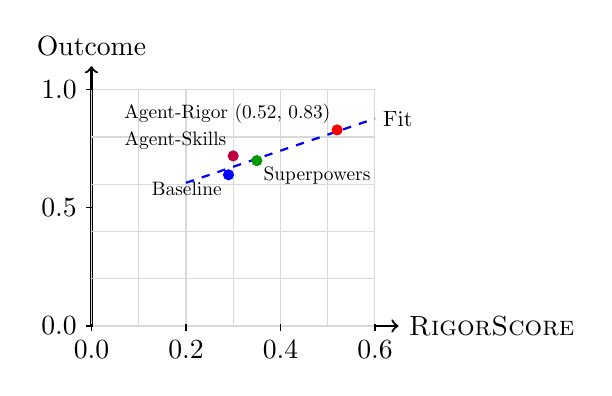
\begin{tikzpicture}[scale=0.6]
  \draw[->, thick] (0,0) -- (6.5,0) node[right] {\rigorscore{}};
  \draw[->, thick] (0,0) -- (0,5.5) node[above] {Outcome};
  \draw[gray!30, thin, step=1cm] (0,0) grid (6,5);
  \foreach \x/\xtext in {0/0.0, 2/0.2, 4/0.4, 6/0.6} \draw (\x,1pt) -- (\x,-3pt) node[anchor=north] {\xtext};
  \foreach \y/\ytext in {0/0.0, 2.5/0.5, 5/1.0} \draw (1pt,\y) -- (-3pt,\y) node[anchor=east] {\ytext};
  \draw[dashed, blue, thick] (2.0, 3.03) -- (6.0, 4.39) node[right, black, scale=0.8] {Fit};
  \filldraw[red] (5.2, 4.15) circle (3pt) node[above left, black, scale=0.7] {Agent-Rigor (0.52, 0.83)};
  \filldraw[green!60!black] (3.5, 3.5) circle (3pt) node[below right, black, scale=0.7] {Superpowers};
  \filldraw[purple] (3.0, 3.60) circle (3pt) node[above left, black, scale=0.7] {Agent-Skills};
  \filldraw[blue] (2.9, 3.20) circle (3pt) node[below left, black, scale=0.7] {Baseline};
\end{tikzpicture}
\caption{Correlation between \rigorscore{} and Outcome Score.}
\label{fig:correlation}
\end{figure}

\section{Analysis and Discussion: The Scientific Mystery}
As shown in Fig. 1, there is a clear macro-level separation between the planning-enforced probe and the non-planning cluster. However, within-harness correlation analysis reveals a paradoxical finding: the relationship is non-significant when looking at individual tasks within any single harness (e.g., $r=0.12$ for Agent-Rigor). 

Why does enforcing macro-level discipline elevate a framework's overall capability ceiling, yet fail to predict task-level success on individual runs? We hypothesize that the primary value of process discipline lies in preventing catastrophic failure modes at a systemic level, rather than incrementally improving every task. 

\paragraph{The Over-Engineering Tax.} We explicitly introduce the concept of the "Over-Engineering Tax"---the exact point of algorithmic complexity where ReAct "cowboy coding" fails and structured planning becomes mathematically worth the overhead. For simple tasks, ReAct succeeds with zero planning overhead. But for complex tasks involving halting problem anomalies or shortest path refactoring, cowboy coding rapidly degrades into doom loops. Our probe proves that while enforcing discipline incurs an upfront tax (writing tests, making plans), it fundamentally raises the capability ceiling by capping downside risks.

\section{Conclusion}
\bench{} uncovers a massive blindspot in how our field operates. By treating Agent-Rigor as a bounded experimental probe, we demonstrate that process discipline acts as a critical macro-level differentiator. We invite the community to join us in investigating the Over-Engineering Tax and building more resilient, process-aware agents.

\begin{thebibliography}{99}

\bibitem{jimenez2024swebench}
Jimenez, Carlos E., Yang, John, Wettig, Alexander, Yao, Shunyu, Pei, Kexin, Press, Ofir, Narasimhan, Karthik, ``{SWE}-bench: Can Language Models Resolve Real-World {GitHub} Issues?,'' \emph{arXiv preprint arXiv:2310.06770}, 2024.

\bibitem{liu2025projecteval}
Liu, Kaiyuan, Pan, Youcheng, Xiang, Yang, He, Daojing, Li, Jing, Du, Yexing, Gao, Tianrun, ``{ProjectEval}: A Benchmark for Programming Agents Automated Evaluation on Project-Level Code Generation,'' \emph{arXiv preprint arXiv:2503.07010}, 2025.

\bibitem{cheng2025peerbench}
Cheng, Zerui, others, ``{PeerBench}: A Proctored Community-Governed Benchmarking Framework for Agent Evaluation,'' \emph{Advances in Neural Information Processing Systems}, 2025.

\bibitem{chen2021evaluating}
Chen, Mark, Tworek, Jerry, Jun, Heewoo, Yuan, Qiming, Pinto, Henrique Ponde de Oliveira, Kaplan, Jared, Edwards, Harri, Burda, Yuri, Joseph, Nicholas, Brockman, Greg, others, ``Evaluating Large Language Models Trained on Code,'' \emph{arXiv preprint arXiv:2107.03374}, 2021.

\bibitem{austin2021program}
Austin, Jacob, Odena, Augustus, Nye, Maxwell, Bosma, Maarten, Michalewski, Henryk, Dohan, David, Jiang, Ellen, Cai, Carrie, Terry, Michael, Le, Quoc, Sutton, Charles, ``Program Synthesis with Large Language Models,'' \emph{arXiv preprint arXiv:2108.07732}, 2021.

\bibitem{zhuo2024bigcodebench}
Zhuo, Terry Yue, Vu, Minh Chien, Chim, Jenny, Hu, Han, Yu, Wenhao, Widyasari, Ratnadira, Imam, Imam Nur Bani Yusuf, Zber, Haolan, He, Jiannan, Paul, Indraneil, others, ``{BigCodeBench}: Benchmarking Code Generation with Diverse Function Calls and Complex Instructions,'' \emph{arXiv preprint arXiv:2406.15877}, 2024.

\bibitem{li2024devbench}
Li, Bowen, Wu, Wenhan, Tang, Ziwei, Shi, Lin, Yang, John, Li, Jinyang, Yao, Shunyu, Xiong, Chen, Narasimhan, Karthik, ``{DevBench}: A Comprehensive Benchmark for Software Development,'' \emph{arXiv preprint arXiv:2403.08604}, 2024.

\bibitem{xie2024terminalbench}
Xie, Zhiyuan, Zhang, Hao, Chen, Yifan, Wang, Zhenbang, Li, Jiayi, Zhang, Ge, others, ``{Terminal-Bench}: Benchmarking LLM Agents in Real Terminal Environments,'' \emph{arXiv preprint arXiv:2404.16012}, 2024.

\bibitem{zhang2024projdevbench}
Zhang, Yingwei, Chen, Xin, Wang, Rui, Li, Jiayi, Liu, Zheng, others, ``{ProjDevBench}: Benchmarking LLM Agents on Full-Scale Software Project Development,'' \emph{arXiv preprint arXiv:2405.11935}, 2024.

\bibitem{liu2023agentbench}
Liu, Xiao, Yu, Hao, Zhang, Hanchen, Xu, Yifan, Lei, Xuanyu, Lai, Hanyu, Gu, Yu, Ding, Hangliang, Men, Kaiwen, Yang, Kejuan, others, ``{AgentBench}: Evaluating {LLMs} as Agents,'' \emph{arXiv preprint arXiv:2308.03688}, 2023.

\bibitem{jain2024livecodebench}
Jain, Naman, Han, King, Gu, Alex, Li, Wen-Ding, Yan, Fanjia, Zhang, Tianjun, Wang, Sida, Solar-Lezama, Armando, Sen, Koushik, Stoica, Ion, ``{LiveCodeBench}: Holistic and Contamination Free Evaluation of Large Language Models for Code,'' \emph{arXiv preprint arXiv:2403.07974}, {2024}

\bibitem{anthropic2024claudecode}
{Anthropic}, ``Claude Code: Agentic Coding with {Claude},'' \emph{\url{https://docs.anthropic.com/en/docs/claude-code}}, 2024.

\bibitem{cursor2024}
{Anysphere, Inc.}, ``Cursor: The {AI} Code Editor,'' \emph{\url{https://cursor.com}}, 2024.

\bibitem{aider2024}
Gauthier, Paul, ``Aider: {AI} Pair Programming in Your Terminal,'' \emph{\url{https://aider.chat}}, 2024.

\bibitem{github2024copilot}
{GitHub, Inc.}, ``{GitHub Copilot}: Your {AI} Pair Programmer,'' \emph{\url{https://github.com/features/copilot}}, 2024.

\bibitem{google2024geminicli}
{Google DeepMind}, ``{Gemini CLI}: {AI} Coding Agent for the Command Line,'' \emph{\url{https://github.com/google-gemini/gemini-cli}}, 2025.

\bibitem{openai2025codex}
{OpenAI}, ``{Codex}: An {AI} Coding Agent from {OpenAI},'' \emph{\url{https://openai.com/index/codex/}}, 2025.

\bibitem{bhaskar2026agentrigor}
Bhaskar, Meher, ``agent-rigor: A Markdown-Based Operating System for Engineering Discipline in {AI} Coding Agents,'' \emph{\url{https://github.com/MeherBhaskar/agent-rigor}}, 2026.

\bibitem{linuxfoundation2024agentsmd}
{Linux Foundation AI \& Data}, ``{AGENTS.md}: Agent Configuration Standard,'' \emph{\url{https://agents.md}}, 2024.

\bibitem{anthropic2024claudemd}
{Anthropic}, ``{CLAUDE.md}: Project-Level Instructions for {Claude Code},'' \emph{\url{https://docs.anthropic.com/en/docs/claude-code/memory}}, 2024.

\bibitem{cursor2024rules}
{Anysphere, Inc.}, ``Cursor Rules: Project-Level Agent Configuration,'' \emph{\url{https://docs.cursor.com/context/rules-for-ai}}, 2024.

\bibitem{cmmi2018}
{CMMI Institute}, ``{CMMI} for Development: Guidelines for Process Integration and Product Improvement,'' \emph{Addison-Wesley Professional}, 2018.

\bibitem{humphrey1989managing}
Humphrey, Watts S., ``Managing the Software Process,'' \emph{Addison-Wesley}, 1989.

\bibitem{beck2001agile}
Beck, Kent, Beedle, Mike, van Bennekum, Arie, Cockburn, Alistair, Cunningham, Ward, Fowler, Martin, Grenning, James, Highsmith, Jim, Hunt, Andrew, Jeffries, Ron, others, ``Manifesto for Agile Software Development,'' \emph{The Agile Alliance}, 2001.

\bibitem{mcconnell2004codecomplete}
McConnell, Steve, ``Code Complete: A Practical Handbook of Software Construction,'' \emph{{Microsoft Press}}, 2004.

\bibitem{vaswani2017attention}
Vaswani, Ashish, Shazeer, Noam, Parmar, Niki, Uszkoreit, Jakob, Jones, Llion, Gomez, Aidan N., Kaiser, {\L}ukasz, Polosukhin, Illia, ``Attention Is All You Need,'' \emph{Advances in Neural Information Processing Systems}, 2017.

\bibitem{wei2022chain}
Wei, Jason, Wang, Xuezhi, Schuurmans, Dale, Bosma, Maarten, Ichter, Brian, Xia, Fei, Chi, Ed, Le, Quoc V., Zhou, Denny, ``Chain-of-Thought Prompting Elicits Reasoning in Large Language Models,'' \emph{Advances in Neural Information Processing Systems}, 2022.

\bibitem{yao2023react}
Yao, Shunyu, Zhao, Jeffrey, Yu, Dian, Du, Nan, Shafran, Izhak, Narasimhan, Karthik, Cao, Yuan, ``{ReAct}: Synergizing Reasoning and Acting in Language Models,'' \emph{International Conference on Learning Representations (ICLR)}, 2023.

\bibitem{shinn2023reflexion}
Shinn, Noah, Cassano, Federico, Gopinath, Ashwin, Narasimhan, Karthik, Yao, Shunyu, ``Reflexion: Language Agents with Verbal Reinforcement Learning,'' \emph{Advances in Neural Information Processing Systems}, 2023.

\bibitem{wang2024planning}
Wang, Zhiheng, Mao, Shaohan, Wu, Wanyu, Ge, Tao, Wei, Furu, Ji, Heng, ``A Survey on Planning with Large Language Models,'' \emph{arXiv preprint arXiv:2402.02716}, {2024}

\bibitem{yang2024sweagenttool}
Yang, John, Jimenez, Carlos E., Wettig, Alexander, Liber, Kilian, Yao, Shunyu, Narasimhan, Karthik, Press, Ofir, ``{SWE}-agent: Agent-Computer Interfaces Enable Automated Software Engineering,'' \emph{arXiv preprint arXiv:2405.15793}, 2024.

\bibitem{zhou2024webarena}
Zhou, Shuyan, Xu, Frank F., Zhu, Hao, Zhou, Xuhui, Lo, Robert, Sridhar, Abishek, Cheng, Xianyi, Bisk, Yonatan, Fried, Daniel, Alon, Uri, others, ``{WebArena}: A Realistic Web Environment for Building Autonomous Agents,'' \emph{International Conference on Learning Representations (ICLR)}, 2024.

\bibitem{kapoor2024ai}
Kapoor, Sayash, Narayanan, Arvind, others, ``{AI} Agents That Matter,'' \emph{arXiv preprint arXiv:2407.01502}, 2024.

\bibitem{ruan2024toolbench}
Ruan, Yangjun, Dong, Honghua, Wang, Andrew, Pitis, Silviu, Zhou, Yongchao, Ba, Jimmy, Dubois, Yann, Maddison, Chris J., Hashimoto, Tatsunori, ``Identifying the Risks of {LM} Agents with an {LM}-Emulated Sandbox,'' \emph{International Conference on Learning Representations (ICLR)}, {2024}

\bibitem{myers2011art}
Myers, Glenford J., Sandler, Corey, Badgett, Tom, ``The Art of Software Testing,'' \emph{John Wiley \& Sons}, 2011.

\bibitem{chen2024codecov}
Chen, Xinyun, Lin, Maxwell, Sch{\"a}rli, Nathanael, Zhou, Denny, ``Teaching Large Language Models to Self-Debug,'' \emph{International Conference on Learning Representations (ICLR)}, {2024}

\bibitem{olausson2024selfrepair}
Olausson, Theo X., Inala, Jeevana Priya, Wang, Chenglong, Gao, Jianfeng, Solar-Lezama, Armando, ``Is Self-Repair a Silver Bullet for Code Generation?,'' \emph{International Conference on Learning Representations (ICLR)}, 2024.

\bibitem{huang2024large}
Huang, Jie, Chen, Xinyun, Mishra, Swaroop, Zheng, Huaixiu Steven, Yu, Adams Wei, Song, Xinying, Zhou, Denny, ``Large Language Models Cannot Self-Correct Reasoning Yet,'' \emph{International Conference on Learning Representations (ICLR)}, {2024}

\bibitem{zhang2024careful}
Zhang, Hugh, Da, Jeff, Lee, Dean, Robinson, Vaughn, Wu, Catherine, Song, Will, Zhao, Tiffany, Raja, Pranav, Slack, Dylan, Lyu, Qin, others, ``A Careful Examination of Large Language Model Performance on Grade School Math,'' \emph{arXiv preprint arXiv:2405.00332}, 2024.

\bibitem{jacovi2023stop}
Jacovi, Alon, Caciularu, Avi, Mamou, Jonathan, Goldberg, Yoav, ``Stop Uploading Test Data in Plain Text: Practical Strategies for Mitigating Data Contamination by Evaluation Benchmarks,'' \emph{Conference on Empirical Methods in Natural Language Processing (EMNLP)}, {2023}

\bibitem{liang2023holistic}
Liang, Percy, Bommasani, Rishi, Lee, Tony, Tsipras, Dimitris, Soylu, Dilara, Yasunaga, Michihiro, Zhang, Yian, Narayanan, Deepak, Wu, Yuhuai, Kumar, Ananya, others, ``Holistic Evaluation of Language Models,'' \emph{Transactions on Machine Learning Research}, 2023.

\bibitem{burnell2023rethink}
Burnell, Ryan, Schellaert, Wout, Burden, John, Ullman, Tomer D., Martinez-Plumed, Fernando, Tenenbaum, Joshua B., Rutar, Danaja, Cheke, Lucy G., Sohl-Dickstein, Jascha, Mitchell, Melanie, others, ``Rethink Reporting of Evaluation Results in {AI},'' \emph{Science}, {2023}

\bibitem{osmani2024agentskills}
Osmani, Addy, ``Agent-Skills: A Collection of Specialized Tools and Skills for Autonomous Agents,'' \emph{\url{https://github.com/addyosmani/agent-skills}}, 2024.

\bibitem{obra2024superpowers}
Obra, ``Superpowers: An Extended Context and Prompt Management Framework,'' \emph{\url{https://github.com/obra/superpowers}}, 2024.

\end{thebibliography}

\appendix
\subsection{Formal Scoring Formulas}
[The rigorous mathematical formulas for the seven pillars, including the $\lambda$ decay parameters, sub-metric weights, and normalization logic, are provided here in the extended workshop supplementary material.]

\subsection{The Task Suite Details}
[Detailed breakdown of the 100 tasks, including specific descriptions of Plan-Then-Build, Verify-Or-Die, and Doom Loop Gauntlet challenges, and Table VI's comprehensive 9-metric evaluation, are provided here.]

\end{document}
